%!TEX root = ../../main.tex

\graphicspath{{../../figures/appendix/}}

\chapter{Convolutional features}
\label{ch:convolutional_features}

\newpage

A paper~\cite{dubois_deep_2019} published at my arrival in the CBIO team proposes to tackle the \ac{RNA} localization problem by learning intermediate features through a convolutional network:

\begin{center}
	\color{green}
	R. Dubois, A. Imbert, et al. (2019), \textit{A Deep Learning Approach To Identify mRNA Localization Patterns}, in 2019 IEEE 16th International Symposium on Biomedical Imaging (ISBI 2019), pp. $\operatorname{1386-1390}$, iSSN: $\operatorname{1945-8452}$.
\end{center}

\noindent
I have participated to this paper by running some experiments to affine the final results, but also by exploring some variants.
Here we present the improvements we obtained with convolutional features and the last results we reached after the paper publication.

\section{Localization features learned with convolutional neural network}
\label{sec:learn_cnn_features}

A deep learning framework presents the advantage to simplify our feature engineering pipeline.
To this end, we directly train a convolutional neural network to classify different localization patterns from a 3-channel image.
Instead of an usual RGB image, we build an input image from the coordinate representation of the cell.
More specifically, we use the \ac{RNA} point cloud (projected in 2D), the 2D cell boundary and the 2D nucleus boundary.
The original paper stacks three layers: one image that assigns to each pixel the number of \ac{RNA}s detected in the pixel, one image with the nucleus boundary and one with the cell boundary.
We also have tested different input designs, replacing the last two boundary images by the binary masks (see figure~\ref{fig:surface_layers}) or the distance map.
Eventually, best results were obtained with binary masks.

\begin{figure}[h]
    \centering
    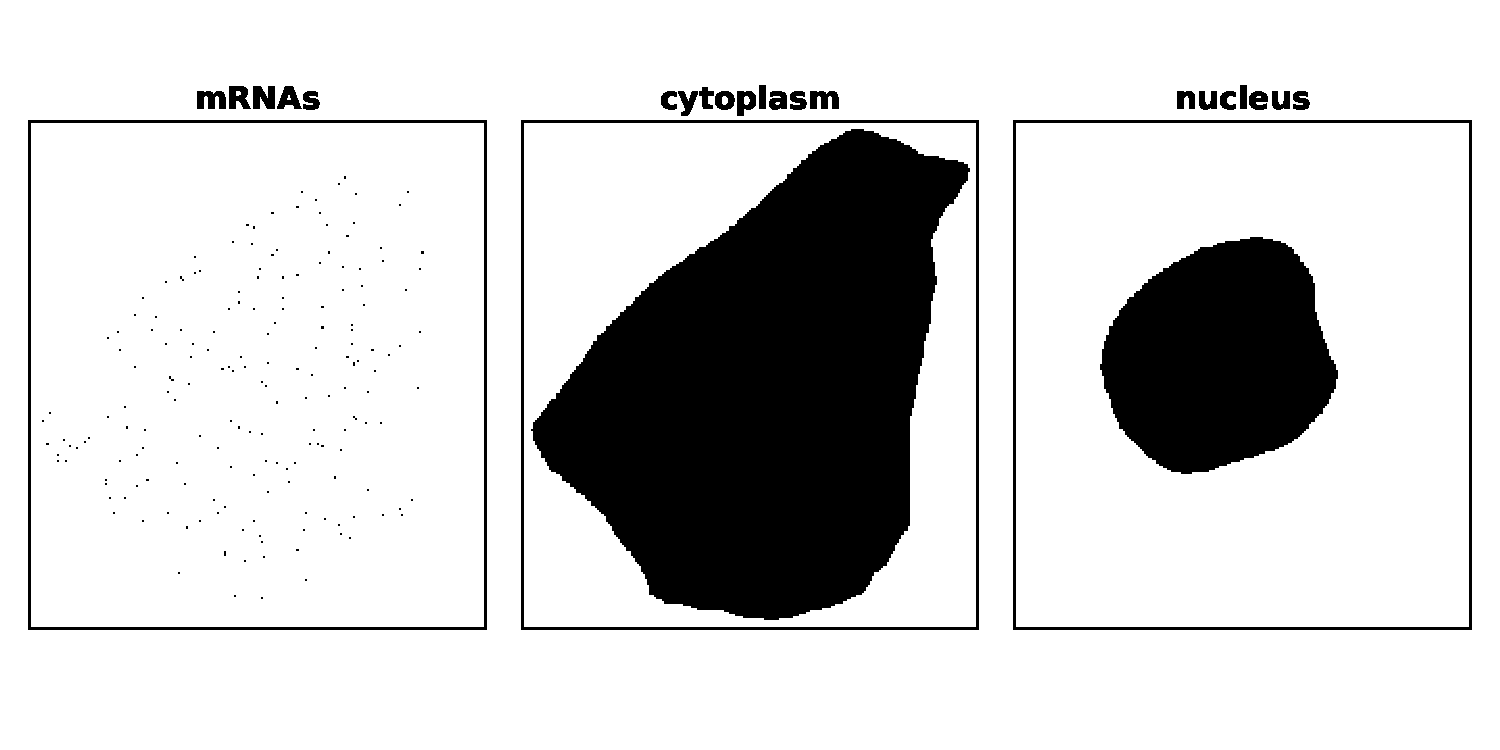
\includegraphics[width=\textwidth]{figures/appendix/surface_layers}
    \caption[Input images for the convolutional model]{Input images for the convolutional model}
    \label{fig:surface_layers}
\end{figure}

Usually, a neural network requires a large annotated dataset to reach good performance and generalized well.
We exploit the MATLAB simulation framework previously released by our group~\cite{samacoits_computational_2018}.
These simulations differ from \emph{simfish}, even if the original 318 cell templates from which we simulate are the same.
In particular, localization patterns and rules to modulate pattern strength are different.
They are greatly simplified in \emph{simfish}.
We simulated 200,000 cells to train, validate and test our model (with a stratified split of 60\%, 20\% and 20\% respectively).
We also use a real dataset with 10 different transcripts visualized across 2791 cells.
Unlike the original paper, we only simulate 5 different patterns: polarization patterns and cell edge were removed because too rare in the real dataset.

We use SqueezeNet~\cite{Iandola_2016} for the image classification task.
This model integrates compression techniques to keep a reasonable accuracy, but drastically reduces the number of parameters to train.
These techniques include squeeze operations to decrease the feature dimension of the layers or a more efficient mix of different convolution kernel sizes.

\section{Results}
\label{sec:results_cnn_features}

\begin{figure}[h]
    \centering
    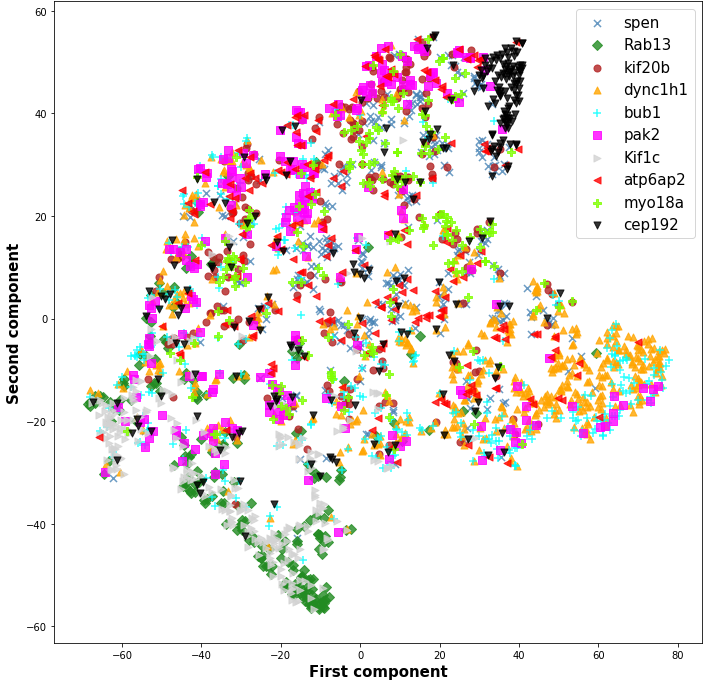
\includegraphics[width=\textwidth]{figures/appendix/tsne_cnn}
    \caption[t-SNE projection of the learned features]{t-SNE projection of the learned features}
    \label{fig:tsne_cnn}
\end{figure}

We can evaluate the classification predictions for the simulated test dataset.
We observe on the confusion matrix~\ref{fig:confusion_matrix_cnn} that the model performs well with the foci pattern, the protrusion pattern (\emph{cellext}) and the intranuclear pattern (\emph{inNUC}).
On the opposite, we fail to predict nuclear edge pattern (\emph{nuc2D}) and random patterns are often confused with foci or intranuclear.
Globally, results are not as good as expected and do not generalize to all the frequent localization patterns observed in the transcriptome.

With the real dataset, we do not have annotations for each cell, but we can still observe more frequent patterns for some genes.
Indeed, the 10 genes selected present a diversity of localization patterns.
We collect the last network layer (before the classification head) and vizualize our cell population with a 2D t-SNE embedding~\cite{vandermaaten_2008,wattenberg2016}.
A first striking observation in figure~\ref{fig:tsne_cnn} is the high level of heterogeneity among the cells (even among the ones labelled with the same \ac{FISH}).
However, distinct clusters can be observed, relevant with the frequent pattern observed with the genes like the intranuclear pattern frequently observed with the CEP192, or the protrusion pattern frequent with KIF1C and RAB13.

\begin{wrapfigure}{L}{0.40\textwidth}
  \begin{center}
    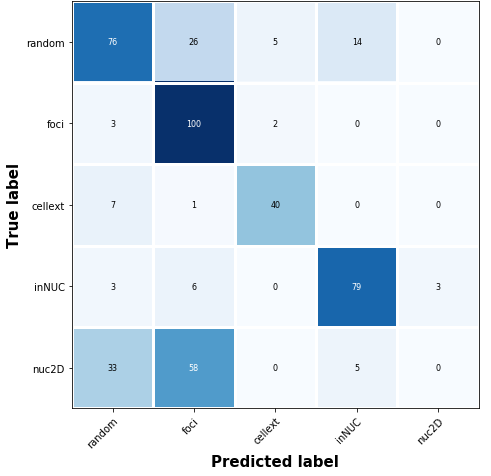
\includegraphics[width=0.33\textwidth]{figures/appendix/confusion_matrix_cnn}
  \end{center}
  \caption[Confusion matrix]{Confusion matrix}
  \label{fig:confusion_matrix_cnn}
\end{wrapfigure}

This study reveals two potential difficulties when we train neural network to learn intermediate features, instead of designing manual ones.
First, when the model makes a prediction, it is much more complicated to understand why it favours a pattern over another.
The internal representation built by the network are not easily accessible or easy to interpret.
There is no direct method to visualize these representations, to quantify the importance of a subregion from the input image in the prediction or to measure the confidence given to a prediction.
However, this is an active field of research and papers~\cite{Yarin_2016,olah2017feature,olah2018the} are investigating it.
Second, by exploiting images of coordinates, we lose a lot of information.
We project a potential 3D \ac{RNA} point cloud in 2D, use an inefficient dense representation (an image) of a sparse input (the \ac{RNA} point cloud) and convolutions might not be the right choice to deals with coordinates inputs~\cite{Rosanne_2018}.